\documentclass{beamer}

\usepackage{amsmath}
\usepackage{amssymb}
\usepackage{amsthm}
\usepackage{amsfonts}

\usepackage{hyperref}
\usepackage{url}

\usepackage{tikz}
\usepackage{color}
\usetikzlibrary{calc,shapes,fadings}


%%%%%%%%%% Tool Names %%%%%%%%%%%%
\newcommand{\pn}{Petri net}
\newcommand{\pns}{Petri nets}
\newcommand{\apical}{$A\pi$-calculus}
\newcommand{\pical}{$\pi$-calculus}
\newcommand{\nest}{\mathit{nest}_\nu}
\newcommand{\depth}{\mathit{depth}}
\newcommand{\set}[1]{\left\{#1\right\}}
\newcommand{\pset}[2]{\set{\,#1\mid#2\,}}
\newcommand{\process}{\mathcal{P}}
\newcommand{\Reach}{\mathit{Reach}}
\newcommand{\subgraph}{\mathrel{\hookrightarrow}}

\newcommand{\tikzMessage}[1]{
  \draw[thick,fill=white] (#1) rectangle ++(0.6, -0.4);
  \path[draw,-,thick] (#1) -- ++(0.3, -0.2) -- ++(0.3, 0.2); 
}
\newcommand{\tikzMessageNode}[2]{
  \node[draw,thick,fill=white,rectangle,inner sep=0pt,minimum height=0.4cm,minimum width=0.6cm] (#1) at (#2) {};
  \path[draw,-,thick] (#2) -- ++(-0.3, 0.2) (#2) -- ++(0.3, 0.2); 
}

\mode<presentation>
{
  \usetheme{Warsaw}
  \useoutertheme{mysplit}
}
% Remove the navigation bar
\setbeamertemplate{navigation symbols}{}

\graphicspath{{./imgs/}}

\title[Ideal Abstraction]{Ideal Abstraction for Well-Structured Transition Systems}

\author{{\bf Damien Zufferey}\inst{1} \and Thomas~Wies\inst{2} \and Thomas A. Henzinger\inst{1}}

\institute{
  \inst{1} IST Austria
  \inst{2} New York University \\
}
\date{VMCAI 2012}

\begin{document}

% Title
\frame[plain]{\titlepage}

%\begin{frame}
%  \frametitle{What are Depth-Bounded Processes (DBP) ?}
%
%  \begin{description}
%  \item[As buzzwords:]
%  concurrent/distributed message-passing programs with process creation and mobility.\\
%  (Warning restrictions may apply.)
%  \item[For the programmers:] some class of programs using the actor model (Erlang, Scala, Akka, ActorFoundry, $\ldots$)
%  \item[For the theoreticians:] a fragment of the $\pi$-calculus.
%  \end{description}
%
%\end{frame}

%\section{Motivation}
\begin{frame}
  \frametitle{Example: client-server communication pattern}
  \begin{figure}
  \centering
  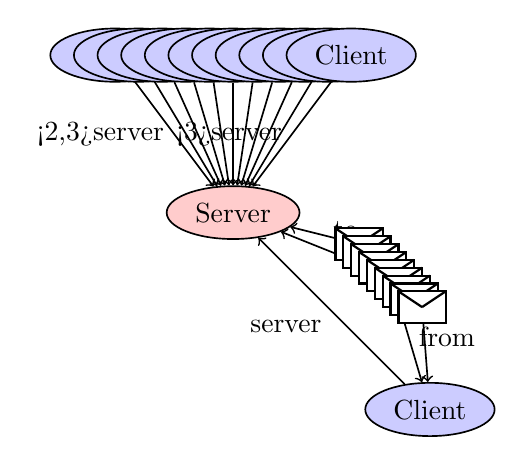
\begin{tikzpicture}[semithick, ->, node distance=2cm]
  \node [draw,ellipse,fill=red!20]  (x) at ( 0, 0) {Server};

  %replication of clients
  \visible<2-> {
  \node [draw,ellipse,fill=blue!20] (ni) at (-1.5, 2) {Client};
  \path  (ni) edge node [left] {\alt<2,3>{server}{}} (x);
  }

  \visible<4-> {
  \node [draw,ellipse,fill=blue!20] (n1) at (-1.2, 2) {Client};
  \path  (n1) edge (x);
  \node [draw,ellipse,fill=blue!20] (n2) at (-0.9, 2) {Client};
  \path  (n2) edge (x);
  \node [draw,ellipse,fill=blue!20] (n3) at (-0.6, 2) {Client};
  \path  (n3) edge (x);
  \node [draw,ellipse,fill=blue!20] (n4) at (-0.3, 2) {Client};
  \path  (n4) edge (x);
  \node [draw,ellipse,fill=blue!20] (n5) at ( 0  , 2) {Client};
  \path  (n5) edge (x);
  \node [draw,ellipse,fill=blue!20] (n6) at ( 0.3, 2) {Client};
  \path  (n6) edge (x);
  \node [draw,ellipse,fill=blue!20] (n7) at ( 0.6, 2) {Client};
  \path  (n7) edge (x);
  \node [draw,ellipse,fill=blue!20] (n8) at ( 0.9, 2) {Client};
  \path  (n8) edge (x);
  \node [draw,ellipse,fill=blue!20] (n9) at ( 1.2, 2) {Client};
  \path  (n9) edge (x);
  }

  \visible<3-> {
  \node [draw,ellipse,fill=blue!20] (nj) at ( 1.5, 2) {Client};
  \path  (nj) edge node [left] {\alt<3>{server}{}} (x);
  }
  
  %replication of messages
  \visible<5-> {
  \node [draw,ellipse,fill=blue!20] (m) at ( 2.5, -2.5) {Client};
  \path  (m) edge node [below left] {server} (x);
  }
  
  \visible<6> {
  \tikzMessageNode{mm}{2.0,-0.8}
  \path  (mm) edge node [right] {from} (m);
  \path  (mm) edge node [above right] {to} (x);
  }

  \visible<7-> {
  \tikzMessageNode{m1}{1.6,-0.4}
  \tikzMessageNode{m3}{1.7,-0.5}
  \tikzMessageNode{m4}{1.8,-0.6}
  \tikzMessageNode{m5}{1.9,-0.7}
  \tikzMessageNode{m6}{2.0,-0.8}
  \tikzMessageNode{m7}{2.1,-0.9}
  \tikzMessageNode{m8}{2.2,-1.0}
  \tikzMessageNode{m9}{2.3,-1.1}
  \tikzMessageNode{m2}{2.4,-1.2}
  \path  (m2) edge (m);
  \path  (m1) edge (x);
  }
  
  \end{tikzpicture}
  \end{figure}
  \visible<8-> {
    This example is a Depth-Bounded Process (DBP),\\
    an instance of WSTS \cite{Meyer08OnBoundednessInDepth,WiesETAL10ForwardAnalysisofDepthBoundedProcesses}.
  }
\end{frame}


\begin{frame}
  \frametitle{What kind of properties are we looking at ?}
  Safety properties, more precisely the control-state reachability problem (aka covering problem).

  \begin{figure}
  \centering
  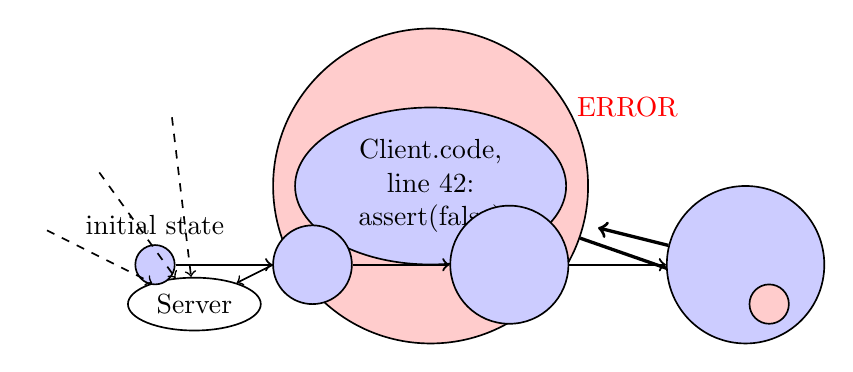
\begin{tikzpicture}[semithick, ->, node distance=2cm]

  \visible<1-2,8> {
  \node[draw,circle,fill=red!20, minimum height=4cm] (err1) at (-0.5,1) {} ;
  \node[color=red] (errlabel) at ( 2, 2) {ERROR};
  \node [draw,ellipse,fill=blue!20,text width=22mm, text centered]  (x) at ( -0.5, 1) {Client.code, line 42: assert(false)};
  \visible<8> {
  \node [draw,ellipse]  (server) at ( -3.5, -0.5) {Server};
  \path  (x) edge (server);
  }
  }

  \visible<2-5> {
  \node[draw,circle,fill=red!20,minimum height=0.5cm]  (err2) at ( 3.8, -0.5) {};
  }
  \visible<2> {
  \path[very thick] (err1) edge (err2);
  }
  \visible<3-6> {
  \node[draw,circle,fill=blue!20,minimum height=0.5cm]  (init) at ( -4, 0) {};
  }
  \visible<3> {
  \node (initlabel) at ( -4, 0.5) {initial state};
  }
  \visible<4-6> {
  \node[draw,circle,fill=blue!20,minimum height=1cm]  (s1) at ( -2, 0) {};
  \path[thick] (init) edge (s1);
  }
  \visible<5-6> {
  \node[draw,circle,fill=blue!20,minimum height=1.5cm]  (s2) at ( 0.5, 0) {};
  \path[thick] (s1) edge (s2);
  }
  \visible<6-8> {
  \node[draw,circle,fill=blue!20,minimum height=2cm]  (s3) at ( 3.5, 0) {};
  \visible<6>{\path[thick] (s2) edge (s3);}
  \node[draw,circle,fill=red!20,minimum height=0.5cm]  (err2) at ( 3.8, -0.5) {};
  }
  \visible<8> {
  \node (invisible) at (1.5,0.5) {};
  \path[very thick] (s3) edge (invisible);
  \begin{scope}
  \node (cli1) at (-3.8,2) {};
  \node (cli2) at (-4.8,1.3) {};
  \node (cli3) at (-5.5,0.5) {};
  \path [dashed] (cli1) edge (server);
  \path [dashed] (cli2) edge (server);
  \path [dashed] (cli3) edge (server);
  \end{scope}
  }

  \end{tikzpicture}
  \end{figure}

\end{frame}

\begin{frame}
  \frametitle{Outline}
  {\Large
  \begin{itemize}
  \item Motivation
  \end{itemize}
  \begin{itemize}
  \item Formalism
  \end{itemize}
  \begin{itemize}
  \item Ideal abstraction
  \end{itemize}
  \begin{itemize}
  \item Example of set-widening for ideal completion% ($\nabla_{\mathsf{DBP}}$)
  \end{itemize}
  }
\end{frame}



%TODO citation of first work by Finkel
%\section{Formalism}
\begin{frame}
  \frametitle{Formal model: WSTS}
  A well-structured transition system (WSTS)
  is a transition system $\langle S, \rightarrow, \leq \rangle$ such that:
  \begin{itemize}
  \item
    $\leq$ is a well-quasi-ordering (wqo),\\
    i.e. well-founded + no infinite antichain.
  \item
    compatibility of $\leq$ w.r.t. $\rightarrow$\\
    \begin{center}
    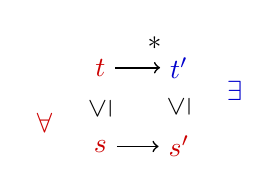
\begin{tikzpicture}[semithick, ->]
    \node[color=red!80!black] (s) {$s$};
    \node[color=red!80!black] (t) [above of=s] {$t$};
    \node[color=red!80!black] (sp) [right of=s] {$s'$};
    \node[color=blue!80!black] (tp) [right of=t] {$t'$};

    \path[color=white]  (s) edge node[color=black,rotate=90] {$\leq$} (t);
    \path  (s) edge (sp);
    \path  (t) edge node [above right] {*} (tp);
    \path[color=white]  (sp) edge node[color=black,rotate=90] {$\leq$} (tp);
    
    \node[color=blue!80!black] (exists) [above right of=sp] {$\exists$};
    \node[color=red!80!black] (forall) [below left of=t] {$\forall$};

    \end{tikzpicture}
    \end{center}
  \end{itemize}

  For more detail see: \cite{DBLP:journals/tcs/FinkelS01, DBLP:conf/lics/AbdullaCJT96}

\end{frame}

%picture about upward and downward closed sets
\begin{frame}
  \frametitle{Downward and upward-closures}
  \begin{figure}
  \centering
  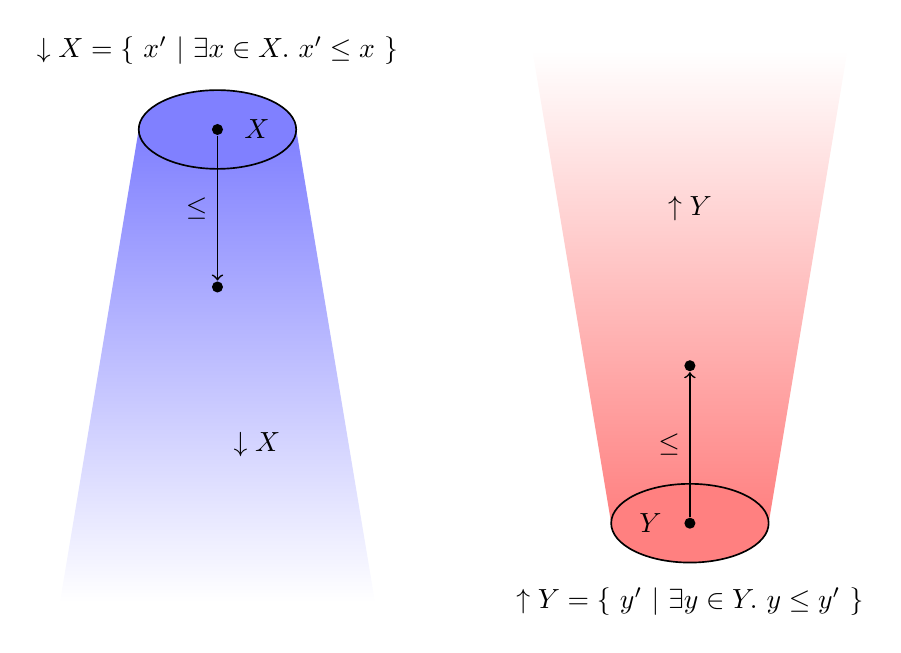
\begin{tikzpicture}[semithick, ->, node distance=2cm]

    \node at (-2,4) {$\downarrow X = \{~ x' ~|~ \exists x \in X.~ x' \leq x ~\}$};
    \shade[top color=blue!50,bottom color=white] (0,-3) -- (-1,3) -- (-3,3) -- (-4,-3);
    \node[draw,ellipse,fill=blue!50,minimum height=1cm,minimum width=2cm] at (-2,3) {};
    \node at (-1.5,3) {$X$};
    \node at (-1.5,-1) {$\downarrow X$};
    \node[fill=black,circle,inner sep=0pt,minimum size=4pt] (d1) at (-2,3) {};
    \node[fill=black,circle,inner sep=0pt,minimum size=4pt] (d2) at (-2,1) {};
    \path (d1) edge node[left] {$\leq$} (d2);
    
    \node at (4,-3) {$\uparrow Y = \{~ y' ~|~ \exists y \in Y.~ y \leq y' ~\}$};
    \shade[bottom color=red!50,top color=white] (2,4) -- (3,-2) -- (5,-2) -- (6,4);
    \node[draw,ellipse,fill=red!50,minimum height=1cm,minimum width=2cm] at (4,-2) {};
    \node at (3.5,-2) {$Y$};
    \node at (4,2) {$\uparrow Y$};
    \node[fill=black,circle,inner sep=0pt,minimum size=4pt] (u1) at (4,-2) {};
    \node[fill=black,circle,inner sep=0pt,minimum size=4pt] (u2) at (4,0) {};
    \path (u1) edge node[left] {$\leq$} (u2);

  \end{tikzpicture}
  \end{figure}
\end{frame}

%TODO not quite efficient -> in the case of DBP (aliasing)
\begin{frame}
  \frametitle{Backward algorithm for covering}
  \begin{center}
  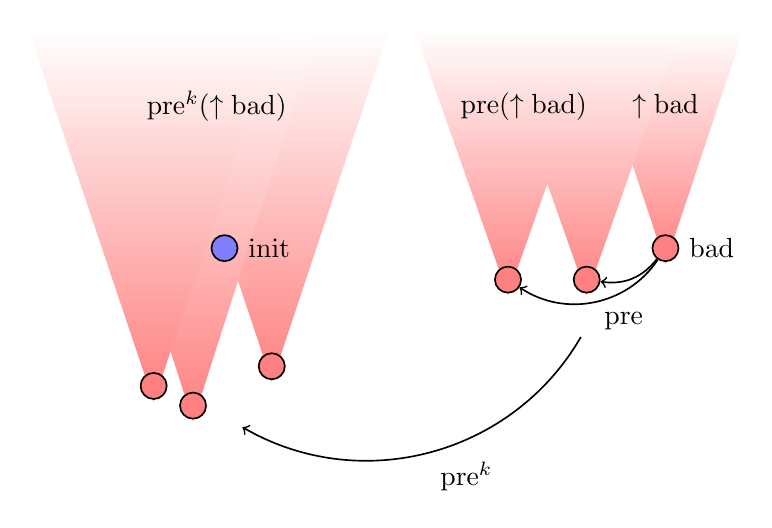
\begin{tikzpicture}[semithick,->]

  \shade[bottom color=red!50,top color=white] (3,5) -- (4,2) -- (5,5);
  \node[draw,circle,fill=red!50,minimum height=0.2,label={right:bad}] (e1) at (4,2.2) {};

  \visible<2->{
  \shade[bottom color=red!50,top color=white] (1.8,5) -- (3,1.6) -- (4.2,5);
  \node[draw,circle,fill=red!50,minimum height=0.2] (e2) at (3,1.8) {};
  \shade[bottom color=red!50,top color=white] (0.8,5) -- (2,1.6) -- (3.2,5);
  \node[draw,circle,fill=red!50,minimum height=0.2] (e3) at (2,1.8) {};
  \path (e1) edge[bend left] (e2);
  \path (e1) edge[bend left=45] node[below right] {pre} (e3);
  \node at (2.2,4) {$\text{pre}(\uparrow\text{bad})$};
  }

  \visible<3->{
  \shade[bottom color=red!50,top color=white] (-2.5,5) -- (-1,0.5) -- (0.5,5);
  \node[draw,circle,fill=red!50,minimum height=0.2] at (-1,0.7) {};
  \shade[bottom color=red!50,top color=white] (-3.6,5) -- (-2,0) -- (-0.4,5);
  \node[draw,circle,fill=red!50,minimum height=0.2] at (-2,0.2) {};
  \shade[bottom color=red!50,top color=white] (-4.1,5) -- (-2.5,0.25) -- (-0.9,5);
  \node[draw,circle,fill=red!50,minimum height=0.2] at (-2.5,0.45) {};

  \node (e4) at (3,1.2) {};
  \node (e5) at (-1.5,0) {};
  \path (e4) edge[bend left=45] node[below right] {pre$^k$} (e5);
  \node at (-1.7,4) {$\text{pre}^k(\uparrow\text{bad})$};
  }

  \visible<4->{
  \node[draw,circle,fill=blue!50,minimum height=0.2,label={right:init}] at (-1.6,2.2) {};
  }
  
  %on top of the shades
  \node at (4,4) {$\uparrow\text{bad}$};
  
  \end{tikzpicture}
  \end{center}
\end{frame}

\begin{frame}
  \frametitle{Forward algorithm for covering}
  \begin{center}
  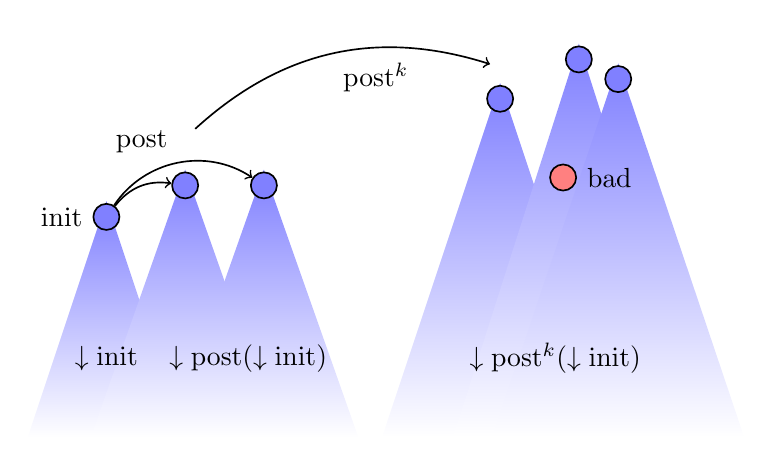
\begin{tikzpicture}[semithick,->]

  \shade[top color=blue!50,bottom color=white] (-3,-5) -- (-4,-2) -- (-5,-5);
  \node[draw,circle,fill=blue!50,minimum height=0.2,label={left:init}] (e1) at (-4,-2.2) {};

  \visible<2->{
  \shade[top color=blue!50,bottom color=white] (-1.8,-5) -- (-3,-1.6) -- (-4.2,-5);
  \node[draw,circle,fill=blue!50,minimum height=0.2] (e2) at (-3,-1.8) {};
  \shade[top color=blue!50,bottom color=white] (-0.8,-5) -- (-2,-1.6) -- (-3.2,-5);
  \node[draw,circle,fill=blue!50,minimum height=0.2] (e3) at (-2,-1.8) {};
  \path (e1) edge[bend left] (e2);
  \path (e1) edge[bend left=45] node[above left] {post} (e3);
  \node at (-2.2,-4) {$\downarrow\text{post}(\downarrow\text{init})$};
  }

  \visible<3->{
  \shade[top color=blue!50,bottom color=white] (2.5,-5) -- (1,-0.5) -- (-0.5,-5);
  \node[draw,circle,fill=blue!50,minimum height=0.2] at (1,-0.7) {};
  \shade[top color=blue!50,bottom color=white] (3.6,-5) -- (2,0) -- (0.4,-5);
  \node[draw,circle,fill=blue!50,minimum height=0.2] at (2,-0.2) {};
  \shade[top color=blue!50,bottom color=white] (4.1,-5) -- (2.5,-0.25) -- (0.9,-5);
  \node[draw,circle,fill=blue!50,minimum height=0.2] at (2.5,-0.45) {};

  \node (e4) at (-3,-1.2) {};
  \node (e5) at (1,-0.3) {};
  \path (e4) edge[bend left] node[below right] {post$^k$} (e5);
  \node at (1.7,-4) {$\downarrow\text{post}^k(\downarrow\text{init})$};
  }

  \visible<4->{
  \node[draw,circle,fill=red!50,minimum height=0.2,label={right:bad}] at (1.8,-1.7) {};
  }
  %on top of the shades
  \node at (-4,-4) {$\downarrow\text{init}$};
  \end{tikzpicture}
  \end{center}
  \visible<5->{
      Computes the covering set rather than answering only a single coverability query.
  }
\end{frame}

%introduce the concept of ideal: 
\begin{frame}
  \frametitle{Representing downward-closed sets with ideals}

  
  \begin{minipage}{0.5\linewidth}
  Given a wqo-set $(X,\leq)$.

  \vspace{10pt}

  A subset of $X$ is \alert{directed} if it is non-empty and closed under upper bounds.
  
  \vspace{10pt}

  An \alert{ideal} of $X$ is a directed downward-closed subset of X.
  
  \vspace{10pt}

  The ideal completion $Idl(X)$ of $X$ is the set of all ideals of $X$.
  \end{minipage}
  \hspace{20pt}
  \begin{minipage}{0.4\linewidth}
  A downward-closed subset is a finite union of ideals.

  \vspace{10pt}

  \begin{center}
  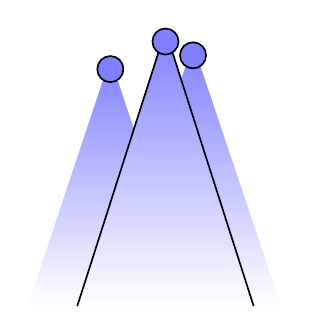
\begin{tikzpicture}[semithick,scale=0.7]
  \shade[top color=blue!50,bottom color=white] (2.5,-5) -- (1,-0.5) -- (-0.5,-5);
  \node[draw,circle,fill=blue!50,minimum height=0.2] at (1,-0.7) {};
  \shade[top color=blue!50,bottom color=white] (4.1,-5) -- (2.5,-0.25) -- (0.9,-5);
  \node[draw,circle,fill=blue!50,minimum height=0.2] at (2.5,-0.45) {};
  \shade[top color=blue!50,bottom color=white] (3.6,-5) -- (2,0) -- (0.4,-5);
  \path[draw] (3.6,-5) -- (2,0) -- (0.4,-5);
  \node[draw,circle,fill=blue!50,minimum height=0.2] at (2,-0.2) {};
  \end{tikzpicture}
  \end{center}
  \end{minipage}
\end{frame}

\begin{frame}
  \frametitle{Ideal for representing downward-closed sets.}
  ADL: \cite{GeeraertsETAL06ExpandEnlargeCheck}\\
  Further developed in \cite{FinkelGoubaultLarrecq09ForwardAnalysisForWSTS}\\
  Applied to DBP in \cite{WiesETAL10ForwardAnalysisofDepthBoundedProcesses}

  \begin{figure}
  \centering
  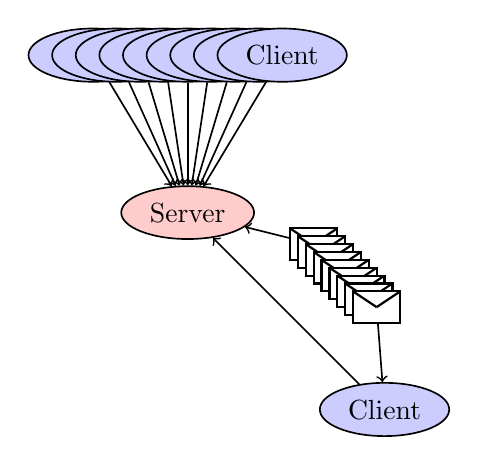
\begin{tikzpicture}[semithick, ->, node distance=2cm]
  \node [draw,ellipse,fill=red!20]  (x) at ( 0, 0) {Server};

  \node [draw,ellipse,fill=blue!20] (n1) at (-1.2, 2) {Client};
  \path  (n1) edge (x);
  \node [draw,ellipse,fill=blue!20] (n2) at (-0.9, 2) {Client};
  \path  (n2) edge (x);
  \node [draw,ellipse,fill=blue!20] (n3) at (-0.6, 2) {Client};
  \path  (n3) edge (x);
  \node [draw,ellipse,fill=blue!20] (n4) at (-0.3, 2) {Client};
  \path  (n4) edge (x);
  \node [draw,ellipse,fill=blue!20] (n5) at ( 0  , 2) {Client};
  \path  (n5) edge (x);
  \node [draw,ellipse,fill=blue!20] (n6) at ( 0.3, 2) {Client};
  \path  (n6) edge (x);
  \node [draw,ellipse,fill=blue!20] (n7) at ( 0.6, 2) {Client};
  \path  (n7) edge (x);
  \node [draw,ellipse,fill=blue!20] (n8) at ( 0.9, 2) {Client};
  \path  (n8) edge (x);
  \node [draw,ellipse,fill=blue!20] (n9) at ( 1.2, 2) {Client};
  \path  (n9) edge (x);

  \node [draw,ellipse,fill=blue!20] (m) at ( 2.5, -2.5) {Client};
  \path  (m) edge (x);
  
  \tikzMessageNode{m1}{1.6,-0.4}
  \tikzMessageNode{m3}{1.7,-0.5}
  \tikzMessageNode{m4}{1.8,-0.6}
  \tikzMessageNode{m5}{1.9,-0.7}
  \tikzMessageNode{m6}{2.0,-0.8}
  \tikzMessageNode{m7}{2.1,-0.9}
  \tikzMessageNode{m8}{2.2,-1.0}
  \tikzMessageNode{m9}{2.3,-1.1}
  \tikzMessageNode{m2}{2.4,-1.2}
  \path  (m2) edge (m);
  \path  (m1) edge (x);

  \end{tikzpicture}
  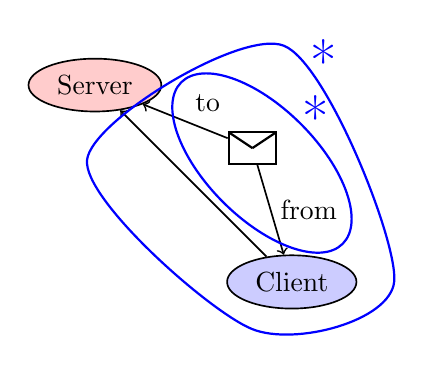
\begin{tikzpicture}[semithick, ->, node distance=2cm]
  \node [draw,ellipse,fill=red!20]  (x) at ( 0, 0) {Server};

  \node [draw,ellipse,fill=blue!20] (m) at ( 2.5, -2.5) {Client};
  \path  (m) edge (x);
  
  \tikzMessageNode{mm}{2.0,-0.8}
  \path  (mm) edge node [right] {from} (m);
  \path  (mm) edge node [above right] {to} (x);

  \draw[thick,rotate=45,color=blue] (0.8,-2.2) ellipse (0.7 and 1.45);
  \node[text=blue] (star) at ( 2.8, -0.4) {{\huge *}};

  \draw[color=blue,thick] plot[smooth cycle] coordinates{(-0.1,-0.95) (2.4,0.5) (3.8,-2.5) (2,-3.1)};
  \node[text=blue] (star) at ( 2.9, 0.3) {{\huge *}};

  \end{tikzpicture}
  \end{figure}
\end{frame}

\begin{frame}
  \frametitle{When does acceleration work ? (flat systems)}

  Forward algorithms are (usually) based on acceleration.

  Acceleration \emph{executes} loops infinitely many time (saturation).

  \vspace{10pt}

  Concretely, The algorithm terminates if the covering set can be generated by executing only simple loops.
  This condition is known as flattability \cite{DBLP:conf/atva/BardinFLS05}.
  Acceleration \emph{executes} traces of length $< \omega^2$.


  
  \begin{figure}
  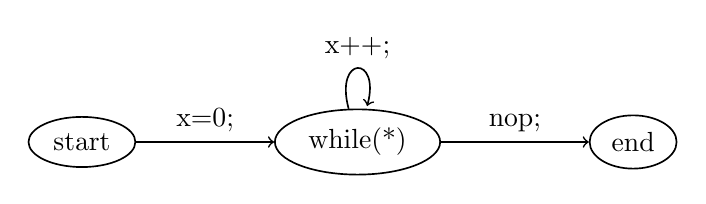
\begin{tikzpicture}[semithick, ->, node distance=35mm]

  \node [draw,ellipse] (loc1) at ( 0, 0) {start};
  \node [draw,ellipse] (loc2) [right of=loc1] {while(*)};
  \node [draw,ellipse] (loc3) [right of=loc2] {end};
  \path  (loc1) edge node[above] {x=0;} (loc2);
  \path  (loc2) edge [loop above] node[above] {x++;}(loc2);
  \path  (loc2) edge node[above] {nop;} (loc3);
  \end{tikzpicture}
  \caption{Example of a flat program}
  \end{figure}

\end{frame}


%\begin{frame}
%  \frametitle{Depth-bounded systems: \cite{Meyer08OnBoundednessInDepth}}
%  System with a bound on the longest acyclic path.\\
%  (Concretely: it is not possible to encode an infinite memory.)
%
%  \vspace{10pt}
%
%  \begin{figure}
%  \centering
%  \begin{tikzpicture}[semithick, ->, node distance=2cm]
%  \node [draw,ellipse,fill=red!20]  (x) at ( 0, 0) {Server};
%
%  \node [draw,ellipse,fill=blue!20] (ni) at (-1.5, 2) {Client};
%  \path  (ni) edge node [left] {} (x);
%  \node [draw,ellipse,fill=blue!20] (n1) at (-1.2, 2) {Client};
%  \path  (n1) edge (x);
%  \node [draw,ellipse,fill=blue!20] (n2) at (-0.9, 2) {Client};
%  \path  (n2) edge (x);
%  \node [draw,ellipse,fill=blue!20] (n3) at (-0.6, 2) {Client};
%  \path  (n3) edge (x);
%  \node [draw,ellipse,fill=blue!20] (n4) at (-0.3, 2) {Client};
%  \path  (n4) edge (x);
%  \node [draw,ellipse,fill=blue!20] (n5) at ( 0  , 2) {Client};
%  \path  (n5) edge (x);
%  \node [draw,ellipse,fill=blue!20] (n6) at ( 0.3, 2) {Client};
%  \path  (n6) edge (x);
%  \node [draw,ellipse,fill=blue!20] (n7) at ( 0.6, 2) {Client};
%  \path  (n7) edge (x);
%  \node [draw,ellipse,fill=blue!20] (n8) at ( 0.9, 2) {Client};
%  \path  (n8) edge (x);
%  \node [draw,ellipse,fill=blue!20] (n9) at ( 1.2, 2) {Client};
%  \path  (n9) edge (x);
%  \node [draw,ellipse,fill=blue!20] (nj) at ( 1.5, 2) {Client};
%  \path  (nj) edge node [left] {} (x);
%  
%  \node [draw,ellipse,fill=blue!20] (m) at ( 2.5, -2.5) {Client};
%  \path  (m) edge node [below left] {} (x);
%  
%  \tikzMessageNode{mm}{2.0,-0.8}
%  \path  (mm) edge node [right] {} (m);
%  \path  (mm) edge node [above right] {} (x);
%
%  \draw[very thick,double] (nj) .. controls (-1,-1) and (2.5,0) .. (m);
%
%  \end{tikzpicture}
%  \end{figure}
%\end{frame}

\begin{frame}
  \frametitle{DBP are intrinsically non-flat.}

  \begin{minipage}{0.6\linewidth}
  initial configuration:
  
  \begin{figure}
  \centering
  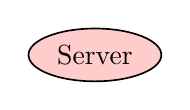
\begin{tikzpicture}[semithick, ->, node distance=2cm]
  \node [draw,ellipse,fill=red!20]  (x) at ( 0, 0) {Server};
  \end{tikzpicture}
  \end{figure}

  covering set:

  \begin{figure}
  \centering
  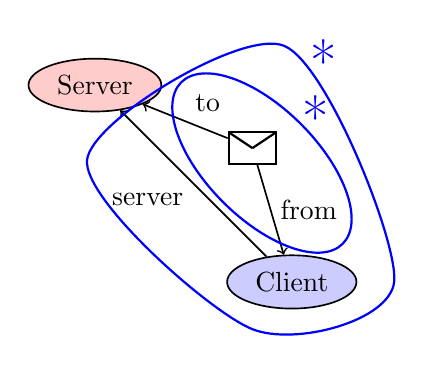
\begin{tikzpicture}[semithick, ->, node distance=2cm]
  \node [draw,ellipse,fill=red!20]  (x) at ( 0, 0) {Server};

  \node [draw,ellipse,fill=blue!20] (m) at ( 2.5, -2.5) {Client};
  \path  (m) edge node [below left] {server} (x);
  
  \tikzMessageNode{mm}{2.0,-0.8}
  \path  (mm) edge node [right] {from} (m);
  \path  (mm) edge node [above right] {to} (x);

  \draw[thick,rotate=45,color=blue] (0.8,-2.2) ellipse (0.7 and 1.45);
  \node[text=blue] (star) at ( 2.8, -0.4) {{\huge *}};

  \draw[color=blue,thick] plot[smooth cycle] coordinates{(-0.1,-0.95) (2.4,0.5) (3.8,-2.5) (2,-3.1)};
  \node[text=blue] (star) at ( 2.9, 0.3) {{\huge *}};

  \end{tikzpicture}
  \end{figure}
  
  \end{minipage}
  \begin{minipage}{0.35\linewidth}
  $\omega^2$ steps from the initial state and the final state.

  \vspace{10pt}

  Nested loops are required to compute the covering set.
  \end{minipage}

\end{frame}

%\section{Ideal Abstraction}
\begin{frame}
  \frametitle{From acceleration to widening}

  Acceleration considers transitions - widening only states.

  \begin{figure}
  \centering
  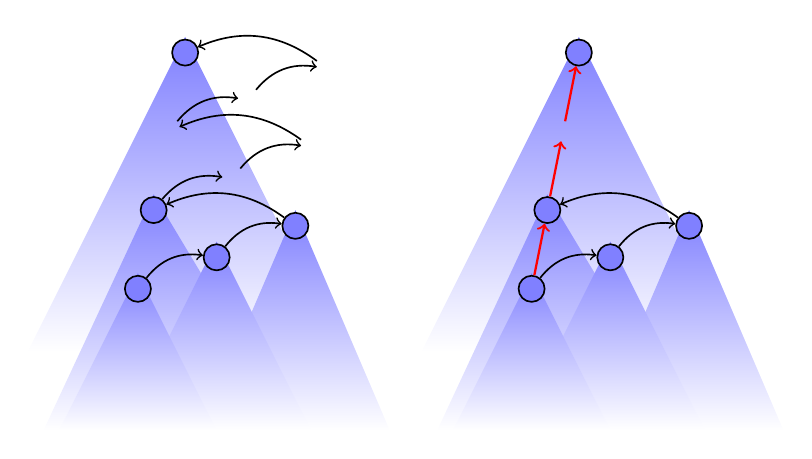
\begin{tikzpicture}[semithick, ->, node distance=2cm]

  \begin{scope}
  
  %layer 1: shades
  \visible<6->{
    \shade[top color=blue!50,bottom color=white] (-1.4,-3) -- (-3.4,1) -- (-5.4,-3);
  }
  \visible<5->{
  }
  \visible<4->{
    \shade[top color=blue!50,bottom color=white] (-2,-4) -- (-3.8,-1.0) -- (-5.2,-4);
  }
  \visible<3->{
    \shade[top color=blue!50,bottom color=white] (-0.8,-4) -- (-2,-1.2) -- (-3.2,-4);
  }
  \visible<2->{
    \shade[top color=blue!50,bottom color=white] (-1.8,-4) -- (-3,-1.6) -- (-4.2,-4);
  }
  \visible<1->{
    \shade[top color=blue!50,bottom color=white] (-3,-4) -- (-4,-2) -- (-5,-4);
  }
  
  %layer 2: nodes
  \visible<1->{
    \node[draw,circle,fill=blue!50] (e1) at (-4,-2.2) {};
  }
  \visible<2->{
    \node[draw,circle,fill=blue!50] (e2) at (-3,-1.8) {};
  }
  \visible<3->{
    \node[draw,circle,fill=blue!50] (e3) at (-2,-1.4) {};
  }
  \visible<4->{
    \node[draw,circle,fill=blue!50] (e4) at (-3.8,-1.2) {};
  }
  \visible<5->{
    \node (e5) at (-2.8,-0.8) {};
    \node (e6) at (-1.8,-0.4) {};
    \node (e7) at (-3.6,-0.2) {};
  }
  \visible<6->{
    \node (e8) at (-2.6,0.2) {};
    \node (e9) at (-1.6,0.6) {};
    \node[draw,circle,fill=blue!50] (e10) at (-3.4,0.8) {};
  }

  %layer 3: edges 
  \visible<1->{
  }
  \visible<2->{
    \path (e1) edge[bend left] (e2);
  }
  \visible<3->{
    \path (e2) edge[bend left] (e3);
  }
  \visible<4->{
    \path (e3) edge[bend right] (e4);
  }
  \visible<5->{
    \path (e4) edge[bend left] (e5);
    \path (e5) edge[bend left] (e6);
    \path (e6) edge[bend right] (e7);
  }
  \visible<6->{
    \path (e7) edge[bend left] (e8);
    \path (e8) edge[bend left] (e9);
    \path (e9) edge[bend right] (e10);
  }
  
  \end{scope}
  
  \begin{scope}[xshift=5cm]
  
  %layer 1: shades
  \visible<12->{
    \shade[top color=blue!50,bottom color=white] (-1.4,-3) -- (-3.4,1) -- (-5.4,-3);
  }
  \visible<11->{
  }
  \visible<10->{
    \shade[top color=blue!50,bottom color=white] (-2,-4) -- (-3.8,-1.0) -- (-5.2,-4);
  }
  \visible<9->{
    \shade[top color=blue!50,bottom color=white] (-0.8,-4) -- (-2,-1.2) -- (-3.2,-4);
  }
  \visible<8->{
    \shade[top color=blue!50,bottom color=white] (-1.8,-4) -- (-3,-1.6) -- (-4.2,-4);
  }
  \visible<7->{
    \shade[top color=blue!50,bottom color=white] (-3,-4) -- (-4,-2) -- (-5,-4);
  }
  
  %layer 2: nodes
  \visible<7->{
    \node[draw,circle,fill=blue!50] (e1) at (-4,-2.2) {};
  }
  \visible<8->{
    \node[draw,circle,fill=blue!50] (e2) at (-3,-1.8) {};
  }
  \visible<9->{
    \node[draw,circle,fill=blue!50] (e3) at (-2,-1.4) {};
  }
  \visible<10->{
    \node[draw,circle,fill=blue!50] (e4) at (-3.8,-1.2) {};
  }
  \visible<11->{
  }
  \visible<12->{
    \node (e7) at (-3.6,-0.2) {};
    \node[draw,circle,fill=blue!50] (e10) at (-3.4,0.8) {};
  }

  %layer 3: edges 
  \visible<7->{
  }
  \visible<8->{
    \path (e1) edge[bend left] (e2);
  }
  \visible<9->{
    \path (e2) edge[bend left] (e3);
  }
  \visible<10->{
    \path (e3) edge[bend right] (e4);
  }
  \visible<11->{
    \path (e1) edge[red,thick] (e4);
  }
  \visible<12->{
    \path (e4) edge[red,thick] (e7);
    \path (e7) edge[red,thick] (e10);
  }
  
  \end{scope}

  \end{tikzpicture}
  \end{figure}

\end{frame}

\begin{frame}
  \frametitle{Ideal abstraction}

  Rephrase analysis in terms of abstract interpretation \cite{CousotCousot77AbstractInterpretation}.

  \begin{itemize}
  \item Concrete domain: sets of configurations ($\mathcal{P}(S)$)
  \item Abstract domain: \alert{ideal completion of $(S,\leq)$} ($\mathcal{P}_{finite}(Idl(S))$)
  \end{itemize}

  \vspace{5pt}

  \begin{itemize}
  \item Concretization function $\gamma$: identity
  \item Abstraction function $\alpha$: \alert{downward-closure}
  \end{itemize}
  $(\alpha,\gamma)$ is a Galois connection.

  \vspace{10pt}

  Covering set is abstract fixed point: $\mu X. \alpha(init) \cup \alpha \cdot post \cdot \gamma (X) $

  \vspace{5pt}

  To guarantee termination we need a widening operator.

\end{frame}

\begin{frame}
  \frametitle{Widening (1)}

  Goal: try to mimic acceleration (when possible), and force termination
  
  \vspace{1ex}

  A set-widening operator ($\nabla$) \cite{CousotCousot92AbstractInterpretationFrameworks} for a poset $S$ is partial function ($\mathcal{P}(S) \rightarrow S$) that satisfies:
  \begin{description}
  \item[Covering]: for all $X \subseteq S$, $x \in X \Rightarrow x \leq \nabla(X)$;
  \item[Termination]: widening of any ascending chain stabilizes.
  \end{description}

  \vspace{1ex}
  Why set-widening rather than the usual pair-widening.

  Reason of using a set-widening operator: we need the history.

\end{frame}

\begin{frame}
  \frametitle{Widening (2)}

  Keeping it simple: need only \alert{set-widening operator on $\mathit{Idl}(S)$}.
  
  It can be lifted to $\mathcal{P}_{finite}(Idl(S))$, using a general construction (details in the paper).

  \vspace{1ex}
  
  We assume that the ordering $S$ is a \alert{better-quasi-ordering} (bqo).\\
  $\Rightarrow$~ Thus, $\mathit{Idl}(S)$ is also a bqo.\\
  $\Rightarrow$~ No infinite antichain in $\mathit{Idl}(S)$.

  \vspace{1ex}
  
  We still need to define the widening on ideals.

  \vspace{1ex}

  We provide concrete operators for
  \begin{itemize}
  \item Petri nets (and monotonic extensions),
  \item Lossy channel systems \cite{DBLP:conf/lics/AbdullaJ93},
  \item Depth-bounded processes (DBP).
  \end{itemize}

\end{frame}

\begin{frame}
  \frametitle{Set-widening for DBP (1)}

  \begin{figure}
  \centering
  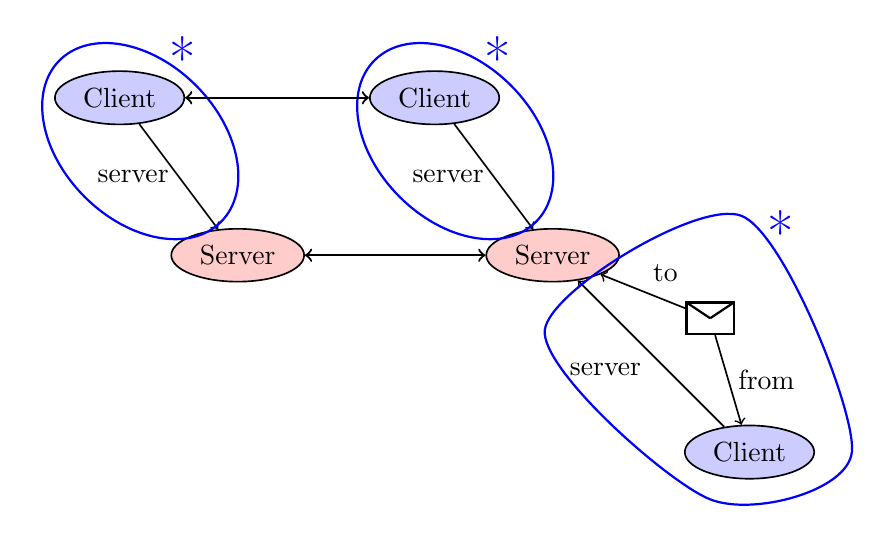
\begin{tikzpicture}[semithick, ->, node distance=2cm]


  \begin{scope}
    \node [draw,ellipse,fill=red!20]  (x) at ( 0, 0) {Server};
    \node [draw,ellipse,fill=blue!20] (ni) at (-1.5, 2) {Client};
    \path  (ni) edge node [left] {server} (x);
    \draw[thick,rotate=45,color=blue] (0.15,1.9) ellipse (1 and 1.45);
    \node[text=blue] (star) at ( -0.7, 2.5) {{\huge *}};
  \end{scope}
  
  \begin{scope}[xshift=4cm]
    \node [draw,ellipse,fill=red!20]  (x2) at ( 0, 0) {Server};
    \node [draw,ellipse,fill=blue!20] (ni2) at (-1.5, 2) {Client};
    \path  (ni2) edge node [left] {server} (x2);
    \draw[thick,rotate=45,color=blue] (0.15,1.9) ellipse (1 and 1.45);
    \node[text=blue] (star) at ( -0.7, 2.5) {{\huge *}};
    \node [draw,ellipse,fill=blue!20] (m) at ( 2.5, -2.5) {Client};
    \path  (m) edge node [below left] {server} (x2);
    \tikzMessageNode{mm}{2.0,-0.8}
    \path  (mm) edge node [right] {from} (m);
    \path  (mm) edge node [above right] {to} (x2);
  \end{scope}
  
  \visible<2->{
    \path[<->,thick] (x) edge (x2);
    \path[<->,thick] (ni) edge (ni2);
  }
  \visible<3->{
    \draw[color=blue,thick] plot[smooth cycle] coordinates{(3.9,-0.95) (6.4,0.5) (7.8,-2.5) (6,-3.1)};
    \node[text=blue] (star) at ( 6.9, 0.3) {{\huge *}};
  }

  \end{tikzpicture}
  \end{figure}
\end{frame}

\begin{frame}
  \frametitle{Set-widening for DBP (2)}

  \begin{figure}
  \centering
  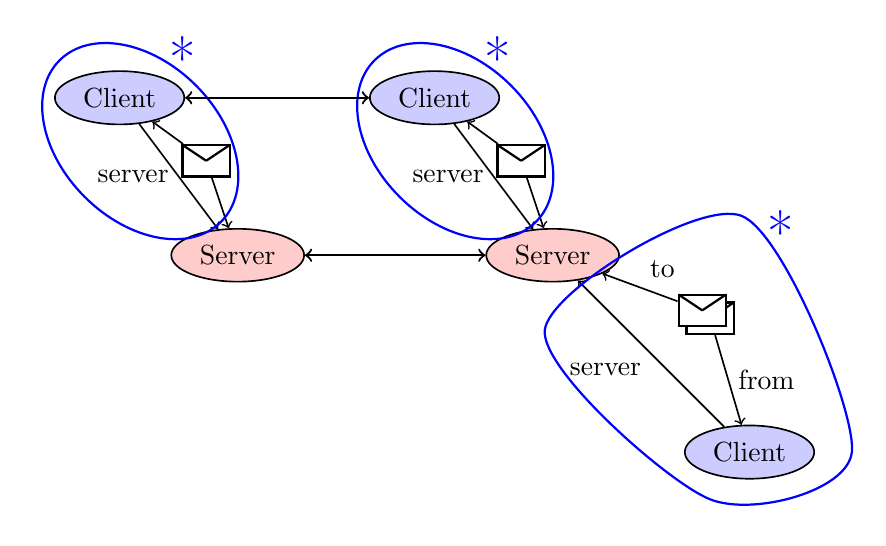
\begin{tikzpicture}[semithick, ->, node distance=2cm]

  \begin{scope}
    \node [draw,ellipse,fill=red!20]  (x) at ( 0, 0) {Server};
    \node [draw,ellipse,fill=blue!20] (ni) at (-1.5, 2) {Client};
    \path  (ni) edge node [left] {server} (x);
    \tikzMessageNode{om}{-0.4,1.2}
    \path  (om) edge (x);
    \path  (om) edge (ni);
    \draw[thick,rotate=45,color=blue] (0.15,1.9) ellipse (1 and 1.45);
    \node[text=blue] (star) at ( -0.7, 2.5) {{\huge *}};
  \end{scope}
  
  \begin{scope}[xshift=4cm]
    \node [draw,ellipse,fill=red!20]  (x2) at ( 0, 0) {Server};
    \node [draw,ellipse,fill=blue!20] (ni2) at (-1.5, 2) {Client};
    \path  (ni2) edge node [left] {server} (x2);
    \tikzMessageNode{om2}{-0.4,1.2}
    \path  (om2) edge (x2);
    \path  (om2) edge (ni2);
    \draw[thick,rotate=45,color=blue] (0.15,1.9) ellipse (1 and 1.45);
    \node[text=blue] (star) at ( -0.7, 2.5) {{\huge *}};
    \node [draw,ellipse,fill=blue!20] (m) at ( 2.5, -2.5) {Client};
    \path  (m) edge node [below left] {server} (x2);
    \tikzMessageNode{mm}{2.0,-0.8}
    \tikzMessageNode{mm2}{1.9,-0.7}
    \path  (mm) edge node [right] {from} (m);
    \path  (mm2) edge node [above right] {to} (x2);
  \end{scope}
  
  \visible<2->{
    \path[<->,thick] (x) edge (x2);
    \path[<->,thick] (ni) edge (ni2);
  }
  \visible<3->{
    \draw[color=blue,thick] plot[smooth cycle] coordinates{(3.9,-0.95) (6.4,0.5) (7.8,-2.5) (6,-3.1)};
    \node[text=blue] (star) at ( 6.9, 0.3) {{\huge *}};
  }

  \end{tikzpicture}
  \end{figure}
\end{frame}

\begin{frame}
  \frametitle{Set-widening for DBP (3)}

  \begin{figure}
  \centering
  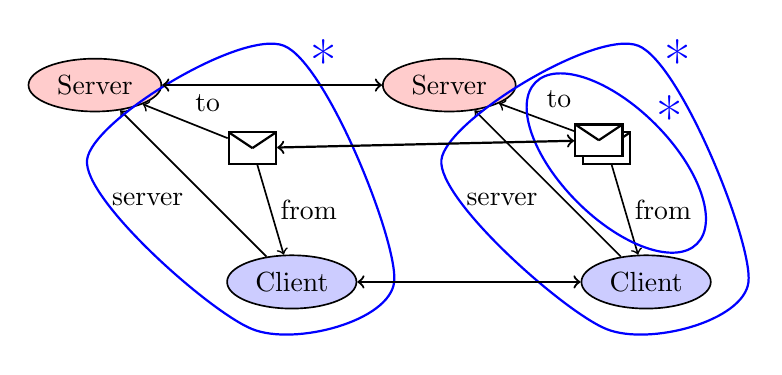
\begin{tikzpicture}[semithick, ->, node distance=2cm]

  \visible<2->{
  \begin{scope}
    \node [draw,ellipse,fill=red!20]  (x) at ( 0, 0) {Server};
    \node [draw,ellipse,fill=blue!20] (m) at ( 2.5, -2.5) {Client};
    \path  (m) edge node [below left] {server} (x);
    \tikzMessageNode{mm}{2.0,-0.8}
    \path  (mm) edge node [right] {from} (m);
    \path  (mm) edge node [above right] {to} (x);
    \draw[color=blue,thick] plot[smooth cycle] coordinates{(-0.1,-0.95) (2.4,0.5) (3.8,-2.5) (2,-3.1)};
    \node[text=blue] (star) at ( 2.9, 0.3) {{\huge *}};
  \end{scope}
  }
  
  \begin{scope}[xshift=4.5cm]
    \node [draw,ellipse,fill=red!20]  (x2) at ( 0, 0) {Server};
    \node [draw,ellipse,fill=blue!20] (m2) at ( 2.5, -2.5) {Client};
    \path  (m2) edge node [below left] {server} (x2);
    \tikzMessageNode{mm1}{2.0,-0.8}
    \tikzMessageNode{mm2}{1.9,-0.7}
    \path  (mm1) edge node [right] {from} (m2);
    \path  (mm2) edge node [above right] {to} (x2);
    \draw[color=blue,thick] plot[smooth cycle] coordinates{(-0.1,-0.95) (2.4,0.5) (3.8,-2.5) (2,-3.1)};
    \node[text=blue] (star) at ( 2.9, 0.3) {{\huge *}};
    \visible<4->{
      \draw[thick,rotate=45,color=blue] (0.8,-2.2) ellipse (0.7 and 1.45);
      \node[text=blue] (star) at ( 2.8, -0.4) {{\huge *}};
    }
  \end{scope}
  
  \visible<3->{
    \path[<->,thick] (x) edge (x2);
    \path[<->,thick] (m) edge (m2);
    \path[<->,thick] (mm) edge (mm2);
  }

  \end{tikzpicture}
  \end{figure}
\end{frame}

\begin{frame}
  \frametitle{Implementation: Picasso}
  Picasso: Pi-Calculus-based Static Software Analyzer

  \vspace{1ex}

  Picasso implements 
  \begin{itemize}
  \item Ideal abstraction domain
  \item Widening for DBP
  \item Trace partitioning domain \cite{DBLP:journals/toplas/RivalM07} (similar to Karp-Miller Tree)
  \end{itemize}

  \vspace{1ex}

  Target: Scala actor programs

  \vspace{0.5ex}

  Input: manually extracted models (soon a compiler plug-in)

  \vspace{0.5ex}
  
  Experimental results in the paper
  
  \vspace{0.5ex}

  Available at \url{http://pub.ist.ac.at/~zufferey/picasso/}.

\end{frame}

\begin{frame}
  \frametitle{Implementation: Results}
{\footnotesize
\begin{tabular}{|l|r|r|r|}
\hline
Name &  tree size & cov.~set size & time \\
\hline
\hline
\texttt{ping-pong} & 17 & 14 & 0.6\,s \\
\hline
\texttt{client-server} & 25 & 2 & 1.9\,s \\
\hline
\texttt{client-server-with-TO} & 184 & 5 & 12.8\,s \\
\hline
\texttt{genericComputeServer} & 57 & 4 & 4.6\,s \\
\hline
\texttt{genericComputeServer-fctAsActor} & 98 & 8 & 14.8\,s \\
\hline
\texttt{liftChatLike} & 1846 & 21 & 1830.9\,s \\
\hline
\texttt{round\_robin\_2} & 830 & 63 & 48.8\,s \\
\hline
\texttt{round\_robin\_3} & 3775 & 259 &  737.8\,s \\
\hline 
\end{tabular}
}
\end{frame}

\begin{frame}
  \frametitle{Further related work:}

  \begin{description}
  \item[\cite{DBLP:conf/lics/AbdullaCJT96}]
  Complete backward algorithm for coverability
  \item[\cite{GeeraertsETAL06ExpandEnlargeCheck}]
  Complete algorithm for coverability based on ideal completions  
  \item[\cite{DBLP:conf/vmcai/GantyRB06}]
  Complete algorithm for coverability based on abstract interpretation but not ideal completions
  \item[\cite{FinkelGoubaultLarrecq09ForwardAnalysisForWSTS}]
  Acceleration-based algorithm for computing covering sets
  \end{description}

\end{frame}

\begin{frame}
  \frametitle{Conclusion}
  \begin{itemize}
  \item Many verification problems for concurrent systems can be phrased in terms of coverability
  \item Coverability is decidable for well-structured transition systems but with high complexity
  \item \alert{Ideal Abstraction}: a generic framework for computing an approximation of the covering set.
    \begin{itemize}
    \item promises precise but more scalable analysis of WSTS
    \item we provide instantiations of the framework for common classes of WSTS
    \item \alert{Picasso}: implementation of our framework for the analysis of Scala actor programs
    \end{itemize}
  \end{itemize}
\end{frame}

\begin{frame}[allowframebreaks]{References}
  \frametitle{}
  {\tiny
  %\bibliographystyle{annotate}
  %\bibliographystyle{plainnat}
  \bibliographystyle{cell}
  %\bibliographystyle{abbrvnat}
  \bibliography{biblio}
  }
\end{frame}

\end{document}
